\documentclass[a4paper,fleqn,usenatbib]{mnras}
\usepackage{txfonts}
\usepackage[T1]{fontenc}
\usepackage{ae,aecompl}
\usepackage{graphicx,color}	% Including figure files
%\usepackage{amsmath}	% Advanced maths commands
\usepackage{amssymb}	% Extra maths symbols
\usepackage{amsbsy}
\usepackage[normalem]{ulem}
\usepackage{mathrsfs,bm,xspace}
\newcommand{\bcdot}{\ensuremath{%
  \mathchoice%
   {\mskip\thinmuskip\lower0.2ex\hbox{\scalebox{1.5}{$\cdot$}}\mskip\thinmuskip}}%
   {\mskip\thinmuskip\lower0.2ex\hbox{\scalebox{1.5}{$\cdot$}}\mskip\thinmuskip}%        
   {\lower0.3ex\hbox{\scalebox{1.2}{$\cdot$}}}%  
   {\lower0.3ex\hbox{\scalebox{1.2}{$\cdot$}}}%
}

% --- macros --- %
\newcommand{\Mstream}{{\it M-streaming}\xspace}
\newcommand{\Mflatturb}{{\it M-turbulence}\xspace}
\newcommand{\Mprimary}{{\it M-primaries}\xspace}

\renewcommand{\vec}{\ensuremath{\mathbfit}}
\newcommand{\dd}{\mathrm{d}}
\newcommand{\Vph}{V_\mathrm{ph}}
\newcommand{\mug}{\mu G}
\newcommand{\RH}{R_\rmn{RH}}
\newcommand{\bvel}{\ensuremath{\boldsymbol{\varv}}}
\newcommand{\bnabla}{\ensuremath{\boldsymbol{\nabla}}}
\newcommand\eb{\epsilon_\rmn{B}}

%\voffset.6in 

\definecolor{mygreen}{rgb}{0.,0.5,0.}
\def\del#1{{}}
%\def\del#1{{\bf (DELETED TEXT)}}
\def\C#1{{\bf #1}}
\def\AP#1{{\bf  AP: #1}}
\def\APP#1{{\bf {\color{red} AP2: #1}}}
\def\SPO#1{{\bf {\color{blue} SPO: #1}}}
\def\CP#1{{\bf {\color{mygreen} CP: #1}}}

\title[Origin of Seed Electrons]{Turbulence and Particle Acceleration in Giant Radio Halos: the Origin of Seed Electrons}  

\author[A. Pinzke, S. Peng Oh and C. Pfrommer] 
{Anders Pinzke$^{1,2}$\thanks{apinzke@fysik.su.se (AP); peng@physics.ucsb.edu (SPO); christoph.pfrommer@h-its.org (CP)}, S. Peng Oh$^{3}$ and Christoph Pfrommer$^{4}$\footnotemark[1]\\
$^{1}$The Oskar Klein Centre for Cosmoparticle Physics, Stockholm University, AlbaNova University Center, SE - 106 91
  Stockholm, Sweden\\
$^{2}$Dark Cosmology Center, University of Copenhagen,
  Juliane Maries Vej 30, DK-2100 Copenhagen, Denmark\\
  $^{3}$University of California - Santa Barbara,
  Department of Physics, CA 93106-9530, USA\\
$^{4}$Heidelberg Institute for Theoretical Studies
  (HITS), Schloss-Wolfsbrunnenweg 35, 69118 Heidelberg, Germany}

\begin{document}
\pagerange{\pageref{firstpage}--\pageref{lastpage}} \pubyear{2015}
\maketitle
\label{firstpage}

%\date{\today}

%\pacs{98.65.Cw, 98.70.Sa, 95.85.Bh, 95.30.Qd, 95.30.Cq, 94.05.Lk, 94.05.Pt}

 
\begin{abstract}
  About one third of X-ray-luminous clusters show smooth, unpolarized
  radio emission on $\sim$Mpc scales, known as giant radio halos. One
  promising model for radio halos is Fermi II acceleration of seed
  relativistic electrons by compressible turbulence in the
  intracluster medium (ICM); Coulomb losses prohibit acceleration from
  the thermal pool. However, the origin of seed electrons has never
  been fully explored. Here, we integrate the Fokker-Planck equation
  of the cosmic ray (CR) electron and proton distributions in
  cosmological simulations of cluster formation. For standard
  assumptions, structure formation shocks lead to a seed electron
  population which produces too centrally concentrated radio
  emission. Instead, we present three plausible scenarios for the seed
  CRs that each can reproduce the spatially flat radio emission
  observed in the Coma cluster. (1) The CR proton-to-electron
  acceleration efficiency $K_\rmn{ep} \sim 0.1$ is assumed to be
  larger than in our Galaxy ($K_\rmn{ep} \sim 10^{-2}$), due to the
  magnetic geometry at the shock. The resulting primary electrons
  dominate the radio emission, which is more extended in comparison to
  radio emission from secondary electrons that result from hadronic CR
  interactions in the ICM. (2) CR protons may stream at the Alfv{\'e}n
  speed to the cluster outskirts when the ICM is relatively
  quiescent. A spatially flat CR proton distribution develops and
  produces the required population of secondary seed electrons. (3)
  The ratio of injected turbulent-to-thermal energy density increases
  significantly with radius, as seen in cosmological simulations. This
  generates a flat radio profile when CRs are reaccelerated even if
  the seed population of CRs is steep with radius. These competing
  non-trivial solutions provide incisive probes of non thermal
  processes in the high-$\beta$ ICM.
\end{abstract} 

%% --- keywords --- %
%\begin{keywords}
%  magnetic fields, cosmic rays, radiation mechanisms: non-thermal, elementary
%  particles, galaxies: cluster: general, Galaxy: fundamental parameters
%\end{keywords}
%%\maketitle

% --- section: Introduction --- %
\section{Introduction}
About one third of X-ray-luminous clusters show smooth, unpolarized
radio emission on $\sim$Mpc scales, known as giant radio halos (RHs)
\citep{2014IJMPD..2330007B}. They appear only in disturbed, merging
clusters and the RH luminosity correlates with the X-ray luminosity
\citep{2001A&A...369..441G,2012A&ARv..20...54F} and the Compton
$y$-parameter \citep{2012MNRAS.421L.112B,2013A&A...554A.140P}. The RHs
show that CR electrons and magnetic fields permeate a large volume
fraction of the intra-cluster medium (ICM). The dominant CR source,
given the smoothness and enormous extent of RHs, is thought to be
structure formation shocks \citep{miniati01,pfrommer08}. At the same
time, plasma processes, the origin of magnetic fields and particle
acceleration in a turbulent, high-$\beta$ plasma like the ICM are not
well understood. Radio halos thus provide an incisive probe of
non-thermal processes in the ICM.

There have been two competing models proposed to explain RHs.  The
radio emitting electrons in the ``hadronic model'' are produced in
inelastic (hadronic) CR proton interactions with protons of the
ambient thermal ICM, which generates pions that eventually decay into
electrons and positrons, depending of the charge of the initial pion
(\citealp{1980ApJ...239L..93D,1999APh....12..169B,2001ApJ...562..233M,
  2004A&A...413...17P,2008MNRAS.385.1211P,ensslin11}). CR protons and
heavier nuclei may have been accelerated and injected into the ICM by
structure formation shocks, active galactic nuclei and galactic
winds. However, the strong bimodality that separates X-ray luminous
clusters into radio-active and radio-quite clusters (and requires a
fast switch on/off mechanism of the RH emission) and the very extended
RH emission at low frequencies in Coma (352~MHz) represent a major
challenge to this model class \citep{brunetti12,2014MNRAS.438..124Z}.

The alternative model for RHs is re-energization of seed suprathermal
electrons by Fermi II acceleration when ICM turbulence becomes
transonic during mergers
\citep{1987A&A...182...21S,1993ApJ...406..399G,2001MNRAS.320..365B,
  2004MNRAS.350.1174B,brunetti07,brunetti11,2015ApJ...800...60M}. Due
to the short radiative cooling time of high-energy relativistic
electrons, the cluster synchrotron emission quickly fades away after a
merger, which naturally explains the observed bimodality of RHs
\cite[see e.g.][]{2013MNRAS.429.3564D,2014MNRAS.443.3564D}.

However, there is a salient piece missing in the turbulent
reacceleration model. It relies heavily on the assumption of an
abundant, volume-filling population of seed suprathermal electrons;
direct Fermi II acceleration from the thermal pool is precluded by
strong Coulomb losses
\citep{2008ApJ...682..175P,2012ApJ...759..113C}. These seeds are
presumed to be either fossil CR electrons (CRes) accelerated by
diffusive shock acceleration (DSA) during structure formation
\citep{1999ApJ...520..529S}, or secondaries injected by hadronic
interaction of CR protons (CRps) with thermal protons
\citep{brunetti11}. While analytic estimates have been made, there has
been no ab initio demonstration that structure formation can lead to
the required abundance of seed electrons with the correct spatial and
spectral characteristics. This is a non-trivial requirement: Coulomb
cooling in dense cluster cores is severe, and DSA fossil electrons may
not survive. On the other hand, for secondaries to constitute the seed
population, the CRp population required in the best-studied case of
the Coma cluster must have a very broad and flat (or even slightly
inverted) spatial profile \citep{brunetti12}, in contrast with the
thermal plasma whose energy density declines steeply with radius. In
Fig.~\ref{fig:Edens} we show that such a distribution is not predicted
by cosmological simulations \cite[see
  also][]{pinzke10,2014MNRAS.439.2662V}. If CRps are predominantly
advected with the cluster plasma, their distribution will be peaked
towards the cluster center and shows a similar characteristics as the
thermal plasma. As a consequence, the distribution of secondary
electrons and the resulting radio synchrotron emission is also peaked
since the hadronic reaction is a two-body scattering process (see
Fig.~\ref{fig:Edens}). Hence, the simulated emission falls short
of the observed extended and flat radio profile of the Coma cluster.

\begin{figure}
  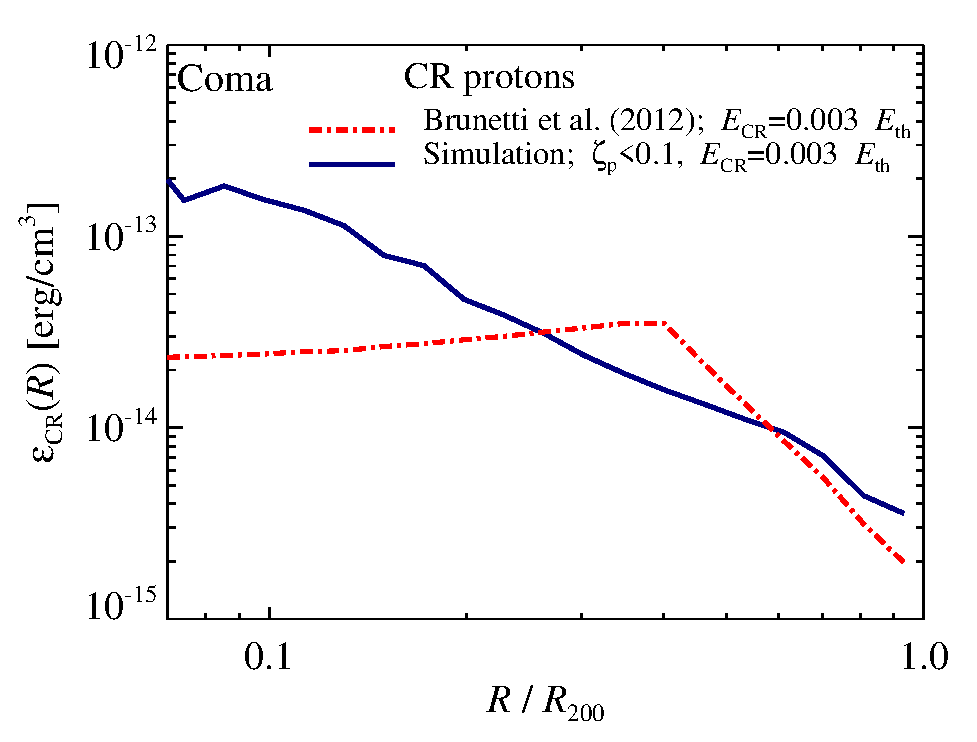
\includegraphics[width=1.0\columnwidth]{fCR.radius.coma.g72a.Rad14.2400p.z0.NL.xKR.eb23.eI067.DII.140.v6.eps}
  \caption{Spatial distribution of CRp energy density in the Coma
    cluster. The red dash-dotted line shows the required distribution
    of seed CRps that generate secondary electrons via p-p collisions
    required to reproduce Coma radio brightness observations after
    Fermi-II reacceleration \citep{brunetti12}. The blue solid line
    shows the distribution of fossil CRps found in cosmological
    simulations, which disagrees with the required profile. To better
    compare the two models in this figure, we normalize the required
    distribution of CRps by fixing the total CRp energy $E_\rmn{CR}$
    to 0.3 percent of the total thermal energy, consistent with
    observations \citep{2014ApJ...787...18A,2012ApJ...757..123A}.}
  \label{fig:Edens}
\end{figure}

Indeed, arriving at a seed population with the required
characteristics is highly constraining, and has the potential to teach
us much about the origin of CRps/CRes in clusters.  In this work, we
use our hydrodynamical zoom simulations of galaxy clusters in a
cosmological setting to follow the distribution functions of seed CRp
and CRe population and integrate the Fokker-Planck equation of CR
transport along Lagrangian particle trajectories. We resolve injection
at structure formation shocks, account for various loss processes of
CRs, and -- most importantly -- model second-order Fermi acceleration
by CR interactions with magnetised turbulence. However, we assume a
simplified and stationary model for magnetic fields and turbulence. We
do not account for the time-varying energy density in compressible
waves, which are thought to be necessary for the acceleration process
\citep{brunetti07,brunetti11}, as the cluster merger proceeds.  So our
approach is orthogonal (and complementary) to e.g.,
\citealp{2015ApJ...800...60M}. This enables us to vary parameters
associated with the unknown continuation of magneto-hydrodynamical
turbulence below the MHD scale and the overall amplitude of
compressible waves.

In this paper we consider three new scenarios that
individually or combined can reproduce the observed radio profiles and
spectrum in the Coma cluster without violating gamma-ray constraints:
\begin{enumerate}
\item {\bf Model {\em M-primaries}.} If the acceleration efficiency of CRps is below
  about $0.1$~{\%} in weak (perpendicular) shocks and the ratio of injected
  electrons-to-protons $K_{\rmn{ep}} \sim 0.1$, this yields a dominant primary
  population with a flat spatial distribution, since primaries have a weaker
  density dependence than secondaries.
\item {\bf Model {\em M-streaming}.} Here, we account for streaming CRps that
  produce flat distributions of CRps in the ICM
  \citep{ensslin11,wiener13,2014MNRAS.438..124Z}, which also flattens the
  secondary electron distribution.
\item {\bf Model {\em M-turbulence}.} Here, we adopt a spatially
  flatter turbulent profile than what was adopted in \citet{brunetti12},
  but where seed CRps follow the steep profile that is suggested by
  structure formation simulations.
\end{enumerate}

To pursue these three possibilities further, we employ cosmological
simulations of CRs in clusters. In tandem with new insights from our
recent work on DSA generated fossil electrons \citep{pinzke13}, we
generate the first quantitative calculation of primary and secondary
seed electrons and compare to observations in the Coma cluster. For
the most part, we adopt parameters that are used in previous work: for
details, see \citep[][ turbulent spectrum]{brunetti07,brunetti11},
\citep[][ injection scale of turbulens]{2015ApJ...800...60M},
\citep[][ energy density of
  turbulence]{2009ApJ...705.1129L,2010ApJ...725.1452S,2011A&A...529A..17V},
for CR acceleration in shocks, \citep[][ in particular $K_{\rmn{ep}}$,
  acceleration efficiency]{pinzke13}, and for cosmological
simulations, \citep[][ i.e., shock history, temperature profile,
  density profile, magnetic field profile]{pinzke10}. All these
parameters are uncertain, and could potentially change our
predictions. We refere the reader to section~\ref{sect:param_comp} for
a small exploration of parameter space, however we leave the full
exploration of parameter space and the interaction between free
parameters to future work.


% --- section: Method --- %
\section{Method} 

The transport of relativistic electrons and protons in
the ICM is a complex process that depends both on the details of the
thermal component (gas density, temperature, and pressure) as well as
non-thermal component (turbulence, magnetic fields, fossil CRs). We
use high resolution galaxy cluster simulations to derive the thermal
and fossil CR properties (shock accelerated primary CRes and CRps, as
well as secondary CRes produced in p-p collisions)
\citep{2007MNRAS.378..385P,pfrommer08,pinzke10,pinzke13}.

[explain overall picture, $\tau_\rmn{d}$ vs. $\tau_{\rmn{cl}}$]


\subsection{Cosmic ray transport}
As previously noted, secondaries produced by shock accelerated CRp
have the wrong spatial profile to explain RH observations; because
they arise from a two body process, they are too centrally
concentrated. They also produce $\gamma$-ray emission in excess of
Fermi-LAT upper limits
\citep{2012ApJ...757..123A,brunetti12,2014ApJ...787...18A}. However,
if CRps stream in the ICM, then their spatial profile could
potentially flatten sufficiently \citep{ensslin11,wiener13}. This
scenario is very attractive: it generates seed electrons with the
right spatial footprint, and by removing CRps from the core, obeys
gamma-ray constraints. Turbulence plays two opposing roles:
Alfv{\'e}nic turbulence damps waves generated by the CR streaming
instability \citep{yan02,farmer04}, thus reducing self-confinement;
but compressible fast modes scatter CRs directly. Turbulent damping is
still efficient for highly subsonic conditions \citep{wiener13}, while
we assume compressible fast modes to only provide effective spatial
confinement during the periods of transonic, highly super-Alfv{\'e}nic
($M_{\rm A} \sim 5$) turbulence associated with mergers. Thus, CRs can
stream out when the cluster is kinematically quiescent. Furthermore,
even Alfv{\'e}nic streaming timescales are relatively short
\cite[$\sim 0.1-0.5$ Gyr;][]{wiener13} compared to the timescale on
which the CRp population is built up. Based on these findings, we
adopt a toy model for our \Mstream scenario in which CR streaming
instantaneously produces flat CRp profiles. \sout{We assume that CRs cannot
stream significantly past perpendicular $B$-fields at the accretion
shock, so that the total number of CRs is conserved within the galaxy
cluster during the streaming process.}

Given a seed population of CRs, we adopt essentially the same set of
plasma physics assumptions as the reacceleration model for RHs
\citep{brunetti07,brunetti11}. We solve the isotropic, gyro-phase
averaged Fokker-Planck equation (via a Crank-Nicholson scheme) for the
time evolution of the CRe distribution in the Lagrangian frame
\citep{brunetti07,brunetti11}:
\begin{eqnarray}
{{d f_{\rmn{e}}(p,t)}\over{d t}} &\!=&
\frac{\partial}{\partial p}
\left\{
f_{\rmn{e}}(p,t)\left[
\left|{{dp}\over{dt}}\right|_{\rm coul} 
+ \frac{p}{3}\left(\bnabla\bcdot \bvel\right)
+ \left|{{dp}\over{dt}}\right|_{\rm r}\right.\right.
\nonumber\\
&-& \left.\left.{1\over{p^2}}{{\partial }\over{\partial p}}\left(p^2 D_{pp}\right) 
\right]\right\} - \left(\bnabla\bcdot \bvel\right) f_{\rmn{e}}(p,t)
- \bnabla\bcdot \vec{F}_\rmn{stream}
\nonumber\\
&+& {{\partial^2 }\over{\partial p^2}}
\left[
D_{pp} f_{\rmn{e}}(p,t) \right]+ Q_{\rmn{e}}\left[p,t;f_{\rmn{p}}(p,t)\right]   \, .
\label{elettroni}
\end{eqnarray}
Here $f_{\rmn{e}}$ is the one-dimensional distribution in position $x$
(suppressed for clarity), momentum $p$ and time $t$ (which is
normalized such that the number density is given by
$n_{\rmn{e}}(t)=\int d p f_{\rmn{e}}(p,t)$), $d/dt=\partial/\partial
t+\bvel\bcdot\bnabla$ is the Lagrangian derivative, $\bvel$ is the gas
velocity, $|dp/dt|$ represents radiative (r) and Coulomb (coul) losses,
$D_{pp}$ is the momentum space diffusion coefficient, and
$Q_{\rmn{e}}$ denotes the injection rate of primary and secondary
electrons in the ICM. The $\bnabla\bcdot \bvel$ terms represent
adiabatic gains and losses and the $\bnabla\bcdot
\vec{F}_\rmn{stream}$ terms represent super-Alfv{\'e}nic CR
streaming. For details about $F_\rmn{stream}$ please see
\citet{wiener13}. During post-processing of our Coma-like cluster
simulation, we solve the Fokker-Planck equation over a redshift
interval from $z=5$ to 0. The simulated cluster undergoes a major
merger over the last 1-2~Gyrs that is thought to inject large
turbulent eddies. Following \citet{brunetti07,brunetti11} \citep[see
  also][]{2004ApJ...614..757Y,2015ApJ...800...60M} we assume that
about one Gyr after core passage the fields have decayed down to the
smallest scales where reacceleration is most efficient ($D_{pp}\sim
k_\rmn{cut}$) and the radio halo turns on shortly after. Note that the
exact decay time of the turbulens is of minor importance, since the
thermal and CR quantities are very similar a few 100 Myrs before and
after $z=0$ where we have chosen to evaluate the simulations. This
delay naturally explains why giant radio halos are only seen in a
fraction of all merging clusters. In all our calculations we assume
that turbulent reacceleration efficiently accelerates particles for
$\tau_\rmn{cl}\sim650$~Myrs (which is roughly the cascade time on which
turbulence is damped) and that during this turbulent phase CR
streaming and spatial diffusion can be neglected. In our \Mstream
model, CR streaming and diffusion are incorporated separately during
kinematically quiescent times that precede the merger. As a result,
flat CRp profiles are produced on relatively short timescales ($\sim
0.1-0.5$ Gyr). This allows us to implicitly solve for CR streaming in
our calculations, where we adopt a toy model that enforce a flat CRp
profile at all quiescent times \citep{wiener13}. We assume that CRs
cannot stream significantly past perpendicular $B$-fields at the
accretion shock, so that the total number of CRs is conserved within
the virial radius during the streaming process. Finally, since
streaming is much more efficient for the CRps, we can ignore this
effect for the CRes.

The time evolution of the spectral energy distribution of CRps,
$f_{\rmn{p}}$, is similarly given by:
\begin{eqnarray}
{{d f_{\rmn{p}}(p,t)}\over{d t}} &=&
{{\partial }\over{\partial p}}
\left\{
f_{\rmn{p}}(p,t)\left[ \left|{{dp}\over{dt}}\right|_{\rm C}
+ \frac{p}{3}\left(\bnabla\bcdot \bvel\right)\right.\right.
\nonumber\\
&-&\left.\left. {1\over{p^2}}{{\partial }\over{\partial p}}\left(p^2 D_{pp}\right)
\right]\right\} - \left(\bnabla\bcdot \bvel\right) f_{\rmn{p}}(p,t)
- \bnabla\bcdot \vec{F}_\rmn{stream}
\nonumber\\
&+& {{\partial^2 }\over{\partial p^2}}
\left[ D_{pp} f_{\rmn{p}}(p,t) \right] - {{f_{\rmn{p}}(p,t)}\over{\tau_{\rm had}(p)}}
+ Q_{\rmn{p}}(p,t)\, ,
\label{eq:FP_p}
\end{eqnarray}
where $Q_{\rmn{p}}(p,t)$ denotes the injection rate of shock
accelerated CRps as a function of momentum $p$ and time $t$, and
$\tau_{\rm had}$ is the timescale of hadronic losses that produce
pions via CRp collisions with thermal protons of the ICM
\cite[e.g.][]{brunetti11}.  


\subsection{Turbulent reacceleration}

We incorporate momentum diffusion for electrons and protons from
transit-time-damping (TTD) resonance with compressible MHD turbulence,
to model Fermi-II reacceleration \citep{brunetti07,brunetti11}. The
TTD resonance requires the wave frequency
$\omega=k_\parallel\upsilon_\parallel$, where $k_\parallel$ and
$\upsilon_\parallel$ are the parallel (projected along the magnetic
field) wavenumber and particle velocity, respectively. This implies
that the particle transit time across the confining wave region
matches the wave period, $\lambda_{\parallel}/v_{\parallel}=T$. Note,
the CRs' gyroradius does not enter the resonance condition. Hence the
CRs that are in resonance with compressible waves experience Fermi-II
acceleration irrespectively of the length scale of the perturbation.

However, the resonance changes the component of particle momentum
parallel to seed magnetic fields, which over time leads to increasing
anisotropy in the particle distribution that decreases the efficiency
of reacceleration with time. As in \citet{brunetti11}, we assume that
there exists a mechanism---such as the firehose instability---that
isotropizes the CR distribution function at the gyroscale and on the
reacceleration time scale, which ensures sustained efficient
reacceleration with time. The particle pitch-angle averaged
momentum-diffusion coefficient of isotropic particles that couple to
fast magnetosonic modes via TTD resonance is \citep[][ Eqn. 47]{brunetti07}:
\begin{eqnarray}
  D_{pp}(p,t) = \frac{\pi}{16} \frac{p^2}{c\,\rho}
  \left\langle\frac{\beta |B_k|^2}{16 \pi \,W}\right\rangle
  I_\theta
  \int_{k_\rmn{cut}}\mathcal{W}(k)k\,d k\,,
\label{eq:dpp}
\end{eqnarray}
where $\beta$ is the thermal-to-magnetic pressure ratio, and $c$
is the speed of light. The energy density $W$ of a mode in a
magnetized plasma stems from both electromagnetic fields and resonant
particles. For a high-$\beta$ plasma, the pitch angle averaged ratio of
beta-weighted magnetic-to-total energy density saturates to $\langle\beta
|B_k|^2/2W\rangle\approx 10^{1.4}$ (see Figure 2 in
\citealt{brunetti07}). The pitch angle of the CR momentum with the
magnetic field orientation is given by $\theta$, and
\begin{equation}
  \label{eq:I_theta}
  I_\theta=\int_0^{\arccos(\Vph/c)} d\theta {\frac{ \sin^3 \theta }{
    |\cos \theta | }}
\left[1+\left(\frac{\Vph}{c\,\cos{\theta}}\right)^2\right]^2.
\end{equation}
Here $V_\rmn{ph}$ is the phase velocity of the fast magnetosonic waves
given approximately by the sound speed, $\Vph \sim c_\rmn{s}$. For a
sound speed typical for the ICM of 1000~km/s, $I_\theta\approx5$. As
in \cite{brunetti07}, we initially assume that the velocity of
turbulent eddies is $V_0\approx 0.47 c_\rmn{s}$ throughout the
cluster. This gives a turbulent acceleration time scale, $\tau_{D} =
p^2/4D_{pp}$, that is typically few 100 Myrs in the ICM (see
Tab.~\ref{tab:timescales} for more details).

We focus on a scenario where the turbulence is injected at the largest
scale that is driven by the merging cluster and accreting matter. The
diffusion equation for isotropic MHD turbulence in $k$--space is given
by
\begin{eqnarray}
&{{\partial {\mathcal W}(k,t) }\over{\partial t}}
=
{{\partial}\over{\partial k}}
\left[
k^2 D_{kk}
{{\partial}\over{\partial k}}
\left( {{ {\mathcal W}(k,t) }\over{k^2}} \right)
\right]
- \sum_i \Gamma_i (k,t) {\mathcal W}(k,t)
+ I(k,t)\nonumber\\
&
\label{modes_kinetic}
\end{eqnarray}
where we assume that the volumetric injection rate of turbulence
$I(k,t)$ is constant over time with a fixed rate $I_0$ so that $I(k,t)
\equiv I(k) = I_0\,\delta (k - k_o)$. The different damping terms are
given by $\Gamma_i(k,t)$ and $D_{kk}$ is the wave--wave diffusion
coefficient of magnetosonic waves in the $k$--space represented by
\begin{equation}
  \label{eq:Dkk}
  D_{kk} \approx \Vph k^4
  \left(\frac{\mathcal{W}(k)}{\rho\,\Vph^2}\right)\,.
\end{equation}

We adopt a simplified isotropic MHD turbulent spectrum based on
Kraichnan's picture for the fast modes per elemental range $dk$ of the
form
\begin{equation}
  \label{eq:Wk}
  \mathcal{W}(k) =
\sqrt{2/7\,I_0\,\rho\,\langle \Vph \rangle}\,k^{-3/2},
\end{equation}
for $k_0<k<k_\rmn{cut}$. Here we adopt a injection scale of the
turbulence, $k_0= 2\pi/(100~\mbox{kpc})$, that is in line with
previous work \citep{brunetti07,brunetti11} \AP{need to be motivated
  beter? why not 1 Mpc}
%, motivated by recent state-of-art simulations \citep{2009A&A...504...33V,2011A&A...529A..17V,2015ApJ...800...60M}.
The profile of injected turbulence is also highly uncertain, however
we assume it correlates to the thermal energy density to some power of
the merging clusters. Hence we assume volumetric injection rate of
turbulent energy, $I_0\propto \epsilon_\rmn{th}^{\alpha_\rmn{tu}}$,
and determine the normalization by requiring that the turbulent energy
in compressible modes $E_\rmn{turb}=\int \int \mathcal{W}(k) \rmn{d}k
\rmn{d}V = X_\rmn{tu} E_\rmn{th}$, where $E_\rmn{th}$ is the total
thermal energy. We adopt a turbulent energy ratio\footnote{Simulations
  show that the compressible modes contribute a factor $0.2-0.4$ to
  the total turbulent energy
  \citep{2013ApJ...771..131B,2015ApJ...800...60M}. Furthermore, the
  total turbulent energy is typically $\sim15-70$\% of the thermal
  energy in a cluster \cite{2011A&A...529A..17V} which is in agreement
  with our adopted value of $X_\rmn{tu}$.}  $X_\rmn{tu}=0.2$ within
the radio halo. In this work we investigate different spatial models
for injected turbulence. With the above choice of normalization, the
turbulent energy density becomes $\epsilon_\rmn{turb} \propto
\epsilon_\rmn{th}^{(\alpha_\rmn{tu}+1)/2}/T^{1/4}$, where $T$ is the
temperature of the gas, $\alpha_\rmn{tu}= 0.67$ for \Mflatturb,
$\alpha_\rmn{tu}= 0.82$ for \Mstream, and $\alpha_\rmn{tu}= 0.88$ for
\Mprimary (see Figure~\ref{fig:turb} for visualisation). Note that in
previous work on the Coma cluster, $\epsilon_\rmn{turb} \propto
\epsilon_\rmn{th}$ was adopted which roughly corresponds to
$\alpha_\rmn{tu}= 1$ \citep{brunetti12} and together with the
different distributions for seed CRes constitute the main differences
compared to our work. Our flatter turbulent profiles are motivated by
fits to cosmological simulations
\citep{2009ApJ...705.1129L,2010ApJ...725.1452S,2011A&A...529A..17V,2012ApJ...758...74B}
and the range indicates uncertainties of the turbulent profile in
Coma. Future observations (by Astro-H) and simulations will help to
clarify this issue. Provided dissipation of turbulence in the ICM is
collisionless, turbulent cascades of compressible modes become
suppressed when thermal and relativistic particles resonantly interact
with magnetosonic waves via TTD on a timescale $\Gamma^{-1}$ that
approaches the cascading timescale given by $\tau_{kk} \approx
k^2/D_{kk}$. Thus, the cascade is suppressed for wave numbers above
\begin{equation}
\label{eq:kc}
  k_\rmn{cut} \approx \frac{81}{14} \frac{I_0}{\rho \langle \Vph \rangle}
  \left(\frac{\langle\sum_i \Gamma_i(k,\theta)\rangle}{k}\right)^{-2}\,,
\end{equation}
where $2\pi/k_\rmn{cut}\sim 0.1-1$~kpc in the ICM. This constitutes an
effective mean free path for CRs, unless plasma instabilities can
mediate interactions between turbulence and particles on smaller
scales \citep{brunetti11}. In this work we only consider damping of
the turbulence via TTD due to thermal electrons, and neglect
subdominant damping with thermal protons and relativistic particles
(conversely, the turbulence has important effects on the
reacceleration of CRs). The latter will be subdominant in the ICM for
a CR-to-thermal energy density ratio $\lesssim 10 \%$
\citep{brunetti07}, which is always satisfied in our models. The
azimuthally averaged turbulent damping rate from thermal electrons
\citep{brunetti07} in a high-$\beta$ plasma is
\begin{equation}
\label{eq:Gamma_e}
\langle\Gamma_{\rmn{e}}\rangle \approx \langle k\,\Vph\,\sqrt{3\pi
  x/20}\exp(-5x/3)\sin^2{\theta}\rangle\approx 0.0435k\,\Vph, 
\end{equation}
where $x=(m_{\rmn{e}}/m_{\rmn{p}})/\cos^2{\theta}$. To compute the
synchrotron surface brightness profiles, we use the profile of the
magnetic field strengths derived from Faraday rotation observations of
Coma \citep{bonafede10} in combination with the density profile
derived from X-ray measurements \citep{1992A&A...259L..31B}.

\begin{figure}
  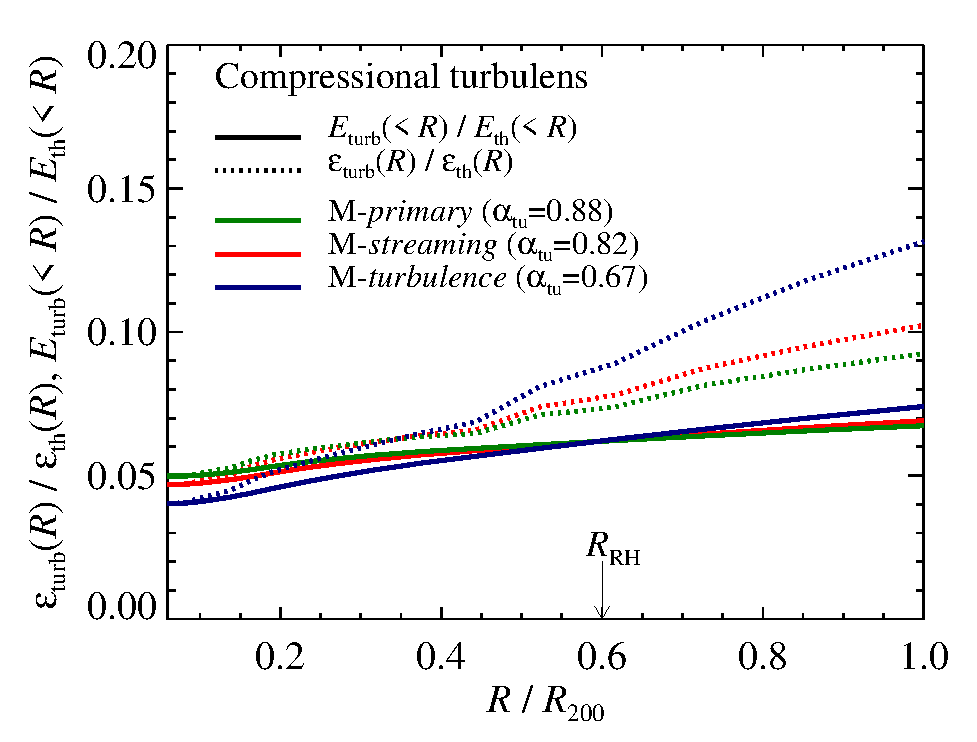
\includegraphics[width=1.0\columnwidth]{turb_profile_ratio_tot.eps}
  \caption{The ratio of turbulent-to-thermal energy densities (solid
    lines) and cumulative energies (dotted lines) in our three
    models. The energy densities are parametrized as
    $\epsilon_\rmn{turb} \propto
    \epsilon_\rmn{th}^{(\alpha_{\rmn{tu}}+1)/2}/T^{1/4}$ and
    normalized such that the total turbulent energy in compressible
    modes $E_\rmn{turb}$ for each scenario makes up about 20\% of the
    total thermal energy $E_\rmn{th}$ inside the radio halo
    ($R_\rmn{RH}\approx0.6R_{200}$). The turbulent profiles explore
    the uncertainty in the cluster turbulence and are motivated by the
    cosmological simulation in
    \citep{2009ApJ...705.1129L,2010ApJ...725.1452S,2011A&A...529A..17V}.}
  \label{fig:turb}
\end{figure}

For reference we show in Table~\ref{tab:timescales} both the thermal
quantities and the timescales for CR cooling and (re)acceleration for
three different spatial regions of the RH. Interestingly the
reacceleration timescale $\tau_D$ is similar between our three models,
where the difference comes from turbulent profile parameterized with
$\alpha_\rmn{tu}$. This implies that even small differences in the
turbulent profile could impact the seed CRs significantly.

\begin{table}
  \caption{Thermal quantities and timescales for different spatial
    regions in a Coma like cluster.}
\begin{tabular}{l c  c c}
\hline
\hline
& & spatial regions & \\
 & $0.1\,\RH^{(2)}$ & $0.3\,\RH^{(2)}$ & $\RH^{(2)}$   \\
\hline
thermal quantities$^{(1)}$ & & & \\
$\rho$ [$10^{-27}$ g cm$^{-3}$] & 3.0 & 1.6 & 0.15 \\
$T$ [$10^{8}$ K] & 1.4 & 1.0 & 0.58 \\
\hline
timescales$^{(1)}$ & & & \\
$\tau_\rmn{D}$(\Mprimary)$^{(3)}$ [Gyr] & 0.45 & 0.44 & 0.39 \\
$\tau_\rmn{D}$(\Mstream)$^{(3)}$  [Gyr] & 0.50 & 0.47 & 0.34 \\
$\tau_\rmn{D}$(\Mflatturb)$^{(3)}$  [Gyr] & 0.69 & 0.56 & 0.27 \\
$\tau_\rmn{IC/sync}(P=10^4\,m_ec)^{(4)}$ [Gyr] & 0.11 & 0.15 & 0.22 \\
$\tau_\rmn{had}(P=100\,m_pc)^{(5)}$ [Gyr] & 2.4 & 4.5 & 47 \\
$\tau_\rmn{coul}(P=\,m_ec)^{(6)}$  [Gyr] & 0.0092 & 0.017 & 0.17 \\
\hline
\end{tabular}
\begin{quote}
 Notes: \\ 
 (1) Median quantities from our simulated post-merging cluster g72a.\\
 (2) Radius of the giant radio halo in Coma where $\RH\approx0.6\,R_{200}$.\\
 (3) Fermi-II reacceleration for both electrons and protons at all energies.\\
 (4) Inverse Compton and synchrotron cooling for electrons.\\
 (5) Catastrophic losses for protons.\\
 (6) Coulomb cooling for electrons (protons factor $m_e/m_p$ smaller).\\

 \label{tab:timescales}
  \end{quote}
\end{table} 


\subsection{Scaling relations for turbulent reacceleratio}
The diffusion constant, $D_\rmn{pp}\propto I_0/\rho c_s \propto
X_\rmn{tu}^2k_0\epsilon_\rmn{th}^{\alpha_\rmn{tu}-1}\sqrt{T}$, where
we adopt the same level of compressible turbulence, $X_\rmn{tu}=0.2$,
for all models. The reaccelerated CRs are exponentially dependent on
this parameter as long as $\tau_D > \tau_\rmn{cl}$, where
$\tau_\rmn{cl}$ represent the duration of reacceleration of the merger
which we assume to be 650~Myrs long. Note that a fixed reacceleration
timescale $\tau_D\sim 1/D_\rmn{pp}\sim 0.2-0.7\,\rmn{Gyr}$ is required
to explain the observations for each model and radial bin (see
Table~\ref{tab:timescales}). This allows us to interchange
$\tau_\rmn{cl} \propto X_\rmn{tu}^2 \propto k_0$, i.e. a longer
reacceleration duration have to be compensated by lowering the level
of turbulence or increasing the physical injection scale of turbulence
to keep $\tau_D$ constant.


\subsection{Spherically symmetric models}
In this section we develope a simple framework that will be used to
test the robustness of our models to the critical parameters for CRs
and turbulence in section~\ref{sect:param_comp}. Here we do not follow
single Lagrangian particles in the cluster, instead we use a more
simple approach where we solve the Fokker-Plack equation in static
spherical shells for injection, reacceleration, and losses of the
CRs. Once the CRs have been reaccelerated for $\tau_\rmn{cl} =
650\,\rmn{Myr}$, we calculate the radio emission and compare the
profile and spectra for different parametrizations.

We adopt both the density \cite{1992A&A...259L..31B} and temperature
\cite{2009ApJ...696.1886B,2001A&A...365L..67A} profiles derived from
X-ray observations of the Coma cluster. They are given by:
\begin{eqnarray}
n_e &=& \frac{3.4\times10^{-3}}{\left[1+\left(R/294\,\rmn{kpc}\right)^2\right]^{1.125}}\nonumber\\
T k_B &=& 8.25\,\rmn{keV} \left[1+\left(R/0.5R_{200}\right)^2\right]^{-0.32}\,.
\end{eqnarray}
The virial radius of Coma is given by $R_{200} = 2300\,\rmn{kpc}$.
The bulk of the CRps are injected by relatively low Mach number shocks
and parametrized by $f_\rmn{CRp,inj}(p) =
C_\rmn{CRp,inj}\,p^{-2.5}$. The CRps trace the thermal gas with
$C_\rmn{CRp,inj} \propto \epsilon_\rmn{th}^{\alpha_\rmn{CR,spat}}$,
where the normalization is fixed by assuming that the injected CR
energy in the last 650~Myrs make up 0.03\% of the thermal energy
inside the virial radius, i.e.
$\int_0^{R_{200}}\epsilon_\rmn{CRp,inj} \rmn{d}
V/\int_0^{R_{200}}\epsilon_\rmn{th} \rmn{d}V = 0.0003$. The spectrum of
  the initial CRp distibtion is determined by the steady state between
  injection and cooling,
\begin{equation}
 f_{CRp,0} \approx \frac{\int_p^\infty f_\rmn{CRp,inj}(p') 
\rmn{d}p'}{\left|{{\rmn{d}p}\over{\rmn{d}t}}\right|_{\rm coul}+\frac{p}{\tau_{\rm had}}}\,,
\end{equation}
where the normalization is fixed by
$\int_0^{R_{200}}\epsilon_\rmn{CRp,inj}
\rmn{d}V/\int_0^{R_{200}}\epsilon_\rmn{th} \rmn{d}V =
0.003$. Similarly, the initial CRe distribution is given by the steady
state between cooling (Coulomb, invers Compton, and synchroton) and
injection of secondary CRes from $f_{CRp,0}$. We also include the
contineous injection of secondary CRes during $\tau_\rmn{cl}$. The
compressible turbulence responsible for reacceleating both the CRps
and CRes is parametrized by $I_0 \propto X_\rmn{tu} (n_e
T)^{\alpha_\rmn{tu}}$. The diffusion constant $D_\rmn{pp}$ is
calculated for each radial bin using
Eqns.~\ref{eq:dpp}-\ref{eq:Gamma_e}. All parameters and assumptions
are similar to what is used for our simulated cluster.

\subsection{Cosmological simulation methodology}
In this paper we focus on our simulated cluster, g72a, which is a
massive $1.6\times10^{15}\,M_\odot$ cluster that experienced a merger
about 1-2 Gyrs ago \citep{2009MNRAS.399..497D}. Since the cluster
mass, density and temperature profiles are all similar to the well
studied Coma cluster \citep{2007MNRAS.378..385P,pinzke10}, we will
compare our calculations to radio and gamma-ray observations of Coma.

We use a simple test-particle model for the CR acceleration and
injection, where each shock inject CRs that trace a power-law in
momentum,
\begin{equation}
  f(p,t) = C(t)\,p^{\alpha_\rmn{inj}}\,,
\end{equation}
determined by the normalization $C(t)$ and the spectral index
$\alpha_\rmn{inj}=\frac{(\gamma_\rmn{ad}+1)\mathcal{M}^2}{(\gamma_\rmn{ad}-1)\mathcal{M}^2+2}$
that depends on the adiabatic index $\gamma_\rmn{ad} = 5/3$ and the
Mach number of the shock $\mathcal{M}$. It is given by the ratio of
the upstream velocity ($u_2$) and the sound speed ($c_s$). The CR
number density and CR energy density are derived from $n_\rmn{CR} =
\int_{p_\rmn{inj}}^\infty \dd p\, f(p)$ and $\epsilon_\rmn{CR} =
\int_{p_\rmn{inj}}^\infty \dd p\, f(p) \,T(p)$, respectively, where
$T(p) = (\sqrt{1+p^2} -1)\, m\,c^2$ is the kinetic energy of a
particle with momentum $p$. We adopt a fit to Monte Carlo
simulations of the thermal leakage process that relates the momentum
of injected protons ($p_\rmn{inj}$) to the thermal energy
($p_\rmn{th}$) of the shocked plasma \citep{kang11}:
\begin{eqnarray}
  \label{eq:qinj}
  p_\rmn{inj} &=& x_\rmn{inj} p_\rmn{th} = x_\rmn{inj} \sqrt{\frac{2 \,k T_2}{m c^2}}\,, \nonumber \\
  \rmn{where}\quad x_\rmn{inj} &\approx& 1.17 \frac{u_2}{p_{\rmn th}\,c} \left(1+
  \frac{1.07}{\epsilon_B}\right) \left(\frac{\mathcal{M}}{3}\right)^{0.1}\,.
\end{eqnarray}
Here $\eb = B_0/B_{\perp}$, $B_0$ is the amplitude of the downstream
MHD wave turbulence, and $B_{\perp}$ is the magnetic field along the
shock normal. The physical range of $\eb$ is quite uncertain due to
complex plasma interactions. In this paper, we adopt $\eb = 0.23$,
which we will later see corresponds to a conservative maximum energy
acceleration efficiency for protons of $10\%$. To derive the
acceleration efficiency, $\zeta_\rmn{inj}$, we first have to infer the
particle injection efficiency, which is the fraction of downstream
thermal gas particles which experience diffusive shock acceleration
\citep[for details see ][]{pinzke13},
\begin{equation}
  \label{eq:eta}
  \eta_\rmn{CR,lin} =
  \frac{4}{\sqrt{\upi}}\,\frac{x_\rmn{inj}^3}{\alpha_\rmn{inj}-1}\,
  \rmn{e}^{-x_\rmn{inj}^2}.
\end{equation}
The particle injection efficiency is a strong function of
$x_\rmn{inj}$ that depends on both $\mathcal{M}$ and $\eb$. The
energy density of CRs that are injected and accelerated at the shock
(neglecting the CR back reaction on the shock) is given by
\begin{equation}
\label{eq:CR_energy} 
  \Delta\epsilon_\rmn{CR,lin} =
  \eta_\rmn{CR,lin}(\mathcal{M})\,T_\rmn{CR}(\mathcal{M},p_\rmn{inj})\,n_\rmn{th}(T_2),
\end{equation}
and the CR energy injection and acceleration efficiency is:
\begin{equation}
  \zeta_\rmn{lin} =
  \frac{\Delta\epsilon_\rmn{CR,lin}}{\Delta\epsilon_\rmn{diss}},
   \quad\mbox{where}\quad
  \Delta\epsilon_\rmn{diss} = \epsilon_\rmn{th2} - \epsilon_\rmn{th0}\,\left(\frac{\rho_2}{\rho_0}\right)^{\gamma_\rmn{ad}}\,.
\label{eqn:energy_frac}  
\end{equation}
The dissipated energy density in the downstream regime,
$\Delta\epsilon_\rmn{diss}$, is given by the difference of the thermal
energy densities in the pre- and post-shock regimes, corrected for the
adiabatic energy increase due to gas compression.

We limit the acceleration efficiency to $\zeta_\rmn{max}$ by
steepening the spectral index of the injected population
$\alpha_\rmn{inj}$ to $\alpha_\rmn{sub}$ so that $\zeta_\rmn{lin}
\leq \zeta_\rmn{max}$ is always fulfilled. The slope
$\alpha_\rmn{inj}$ impact $\zeta_\rmn{inj}$ via the mean energy per
particle given by $T_\rmn{CR} = \epsilon_\rmn{CR}/n_\rmn{CR}$. This
procedure conserves energy and is motivated by models of non-linear
shock acceleration where a sub-shock with a lower compression ratio
(and hence steeper spectral index) forms
\citep[e.g.,][]{2000ApJ...540..292E}. Given our assumed $\eb=0.23$, we
find that for strong shocks where $\alpha \lesssim 2.3$ the spectral
slope is steepened by a maximum of $\sim 10$ per cent in low
temperature regimes ($kT\sim 0.1$~keV), while the steepening is much
smaller for high temperature regimes ($kT\sim 10$~keV) that are more
relevant for clusters. Since $p_\rmn{inj}$ remains fixed, so does the
CR number density $n_\rmn{CR}$. Hence we can solve for the
renormalized normalization constant $C_\rmn{sub}$ using $n_\rmn{CR}$
and Eqn.~\ref{eq:eta}:
\begin{equation}
  \label{eq:Cp_sub}
  C_\rmn{sub}=\eta_\rmn{CR,lin}\,(\alpha_\rmn{sub}-1)\,p_\rmn{inj}^{\alpha_\rmn{sub}-1}\,,
\end{equation}
where the new distribution function is given by $f(p,t)= C_\rmn{sub}
p^{-\alpha_\rmn{sub}}$. We set an upper limit on the ratio of
accelerated proton-to-dissipated energy in the downstream of strong
shocks that varies from $\zeta_\rmn{max} \sim 1-10\%$, depending on
the adopted model (for more details, see Section \ref{sec:results}).

In our Galaxy, the CRe-to-CRp ratio at a few GeV is $K_{\rmn{ep}} \sim
10^{-2}$. Hence, we adopt this as a fiducial value for the CRe-to-CRp
acceleration efficiency (see \cite{pinzke13} for more
discussion). However, as recent PIC simulations have shown, this is
likely very different at weak shocks, with electrons efficiently
accelerated at perpendicular shocks
\citep{2014ApJ...794..153G,2014ApJ...797...47G}, and ions efficiently
accelerated at parallel shocks \citep{2014ApJ...783...91C}. Thus,
depending on magnetic geometry, $K_{\rmn{ep}}$ could be either larger
or smaller. Some observations of radio relics suggest high values of
$K_{\rmn{ep}}$, due to the absence of gamma-ray emission, which probes
the CRp population \citep{2014MNRAS.437.2291V}. This suggests primary
CRes as a viable alternative scenario to secondary CRes as seeds for
the giant RHs. In our {\em M-primaries} scenario, the injected
distribution of CRes is derived in the same way as for the CRps. Once
they have been accelerated to relativistic energies, injected
electrons and protons are indistinguishable. We therefore assume that
CRp and CRe have the same distribution function $f_\rmn{CRe}(p) =
K_\rmn{ep} f_\rmn{CRp}(p)$, with a different normalization (due to
differing acceleration efficiencies) $K_\rmn{ep}=0.1$ \citep[which is
  viable for primarily perpendicular
  shocks][]{2014ApJ...794..153G}. While this appears to contradict the
radial bias of magnetic fields in the bulk of the ICM as suggested by
observations \citep{2010NatPh...6..520P} and cluster simulations
\citep{2011ApJ...740...81R}, it does not necessarily apply to the
accretion shock regions, which show a field geometry with a net
perpendicular bias with respect to the shock normal---at least for
giant radio relics \citep{2010Sci...330..347V}.


% --- section: Analytical Results and discussion --- %
\section{Parameter space exploration with spherical models}
\label{sect:param_comp}
in this paper we rely on several critical parameters decribing
relatively unknown non-thermal physics in the ICM. Here we try to
explore the robustness of our models to the most critical parameters
related to turbulence and CRs. Figure~\ref{fig:param_comp} shows their
impact on radio emission. We find that the level of turbulence
($X_\rmn{tu}$) has a large impact on both radio spectra and profile,
while the parameter $\alpha_\rmn{tu}$ that determines the spatial
profile of turbulence mainly influence the radio profiles. As
expected, the radio profiles flatten significantely with a flatter
turbulent profile. A higher amount of energy also flatten the radio
profile, where the reason beeing that the steep profiles of injected
CRs have less impact on the radio emission for an increasing
reacceleration efficiency. Interestingly, assumptions about CRs have
less impact on radio emission. This can be understood by looking at
the scaling of parameters to the reacceleration timescale, where
$\tau_\rmn{D} \propto X_\rmn{tu}^2$. The CRps approximately gain a
factor $\Delta C_\rmn{reacc.} \sim
\exp{\left[\frac{(2+\alpha)(1-\alpha)}{4}\frac{\tau_\rmn{cl}}{\tau_\rmn{D}}\right]}$
during reacceleration if injection and cooling are neglected. The CRes
gain a similar factor from reacceleration, however in the region
around $0.1\,R_{200}$ the Coulomb cooling timescale
($\tau_\rmn{coul}\approx0.01\,\rmn{Gyr}$) is much shorter than
$\tau_\rmn{D}\approx0.5\,\rmn{Gyr}$, hence $\Delta C_\rmn{reacc.}$
will be greatly reduced for the electrons. The spatial region is
important when we derive the radio spectrum, since in order to compare
to observations we integrate the CR profile out to $\sim
0.2\,R_{200}$. For a CRp spectral index $\alpha_\rmn{CR}\sim 2.5$,
$\Delta C_\rmn{reacc.} \sim
\exp{\left[1.7\frac{\tau_\rmn{cl}}{\tau_\rmn{D}}\right]} \sim 10$ for
$X_\rmn{tu}=0.2$ and $\alpha_\rmn{tu}=0.8$. This is confirmed by the
top panels in Fig.~\ref{fig:param_comp}. Increasing the level of
turbulence to $X_\rmn{tu}=0.3$, gives us a $\Delta C_\rmn{reacc.}
\sim 100$, which is roughly confirmed by same figures. The factor 2-3
difference in the figure is due to the shorter reacceleration
timescale that increase the contribution from reaccelerated CRes that
would othervise cool away on a much shorter timescale. Hence we
conclude that the radio emission is much more sensitive to the
exponential dependence on compressible turbulence than the linjear
dependence on injected CRs. \AP{Too complicated? Perhaps cut or
  simplify?} 

We can also find a lower critical level of turbulence where
reacceleration is negliable, while it rises sharply above this
threshold. We define the threshold by $\Delta C_\rmn{reacc.}  \lesssim
2$, which gives us an $X_\rmn{thres,tu} = \left(\frac{\log(2)
  0.04}{1.7}\frac{\tau_\rmn{D}}{\tau_\rmn{cl}}\right)^{0.5} \approx 0.08$ for
$\tau_\rmn{D} = 0.5\,\rmn{Myr}$. This threshold is also seen in the
top panels of figure~\ref{fig:param_comp}. For instance, for
$X_\rmn{tu}\gtrsim0.08$, a factor two change in $X_\rmn{tu}$ changes
the radio surface brightness by a factor $\sim 10-100$. In principle
this threshold behavior allows us to provide a strict lower bound on
turbulence in radio halos. An even more stringent bound on
$X_\rmn{tu}$ can be inferred from combining radio observations with
the gamma-ray observations (see section~\ref{sect:radio_spec}).

\begin{figure*}
\begin{minipage}{1\columnwidth}
   \begin{center}\Large{Radio profiles}\\
     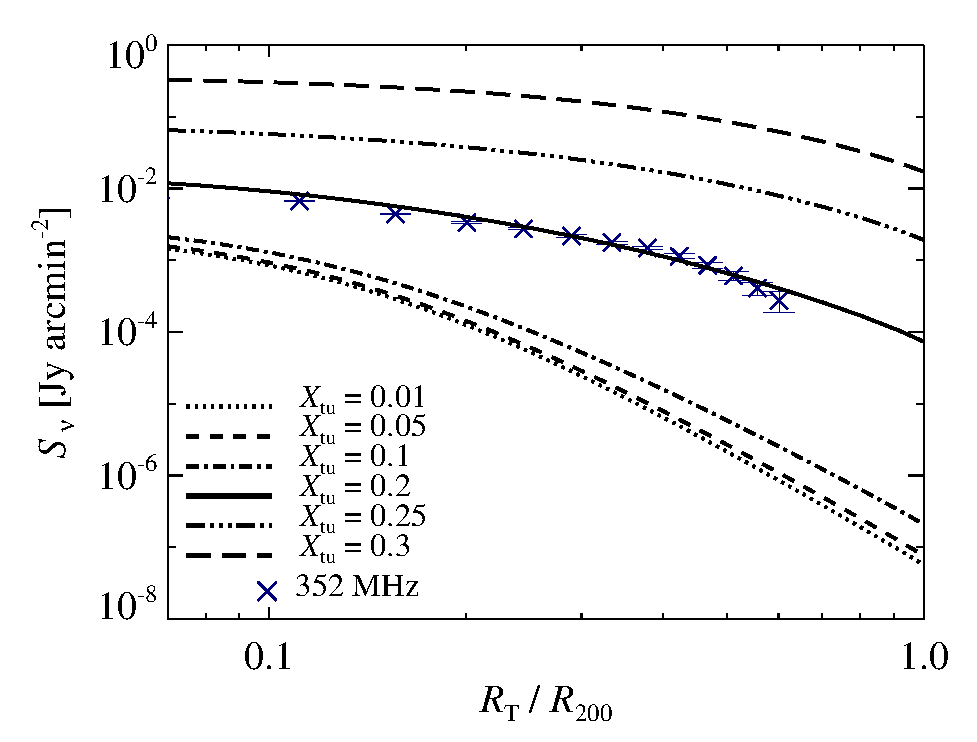
\includegraphics[width=\columnwidth]{prof.comp.KrTTDth.Xtu.eps}
   \end{center}
\end{minipage}
\begin{minipage}{1\columnwidth}
   \begin{center}\Large{Radio spectra}\\
     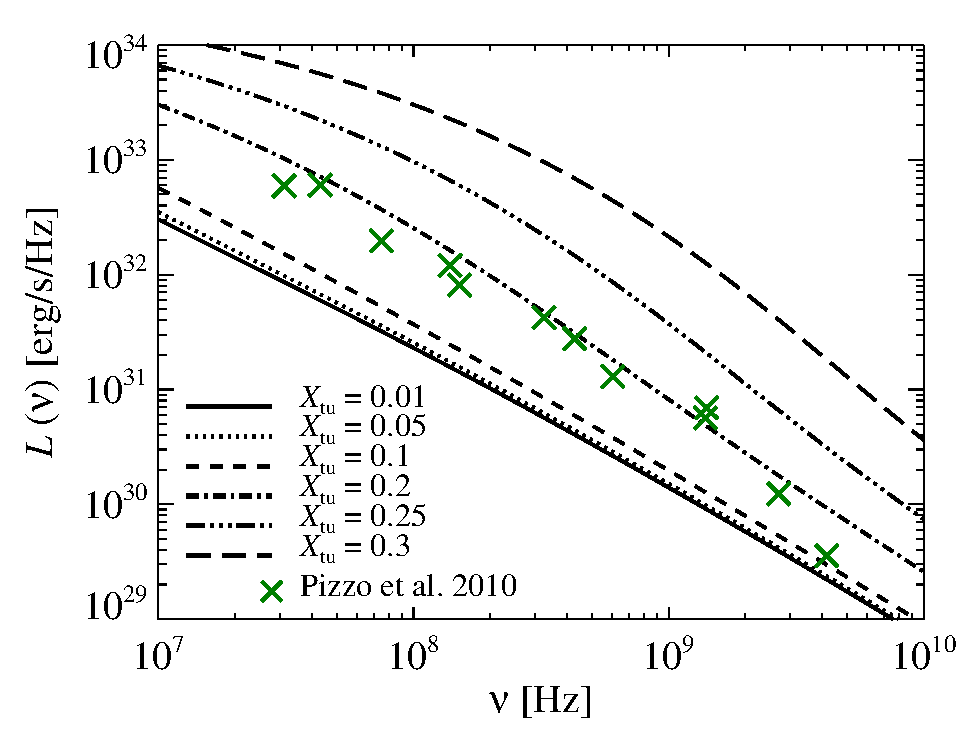
\includegraphics[width=\columnwidth]{spec.comp.KrTTDth.Xtu.eps}
   \end{center}
\end{minipage}
\\
\begin{minipage}{1\columnwidth}
  \begin{center}%\Large{\Mflatturb:}\\ 
    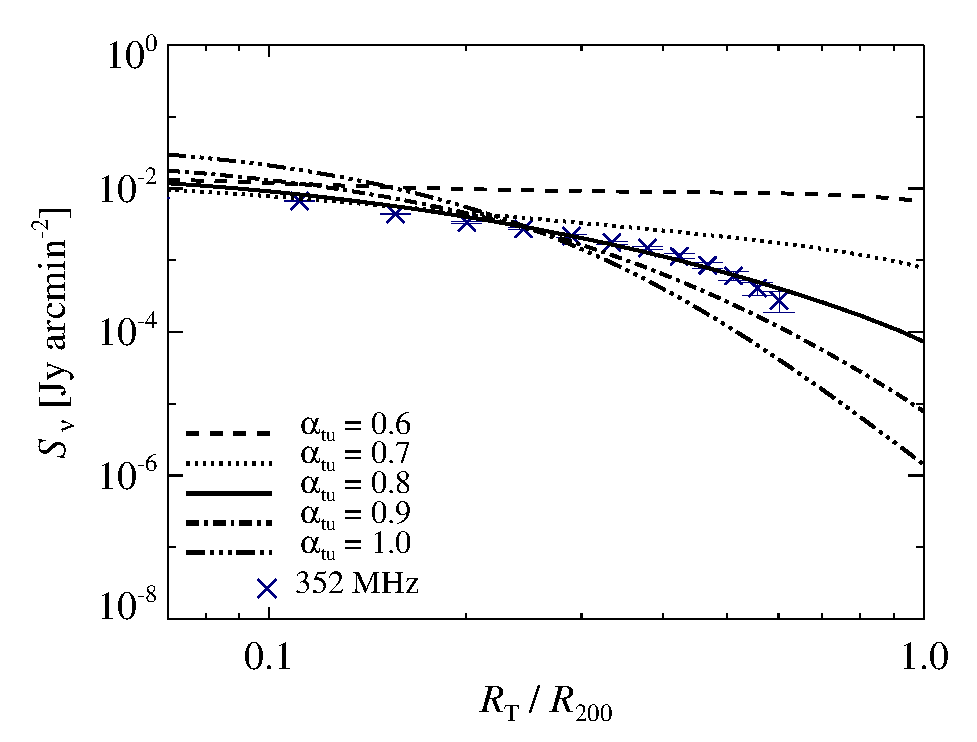
\includegraphics[width=\columnwidth]{prof.comp.KrTTDth.aI0.eps}
  \end{center}
\end{minipage}
\begin{minipage}{1\columnwidth}
   \begin{center}%\Large{\it Brunetti et al. (2012)}:\\
     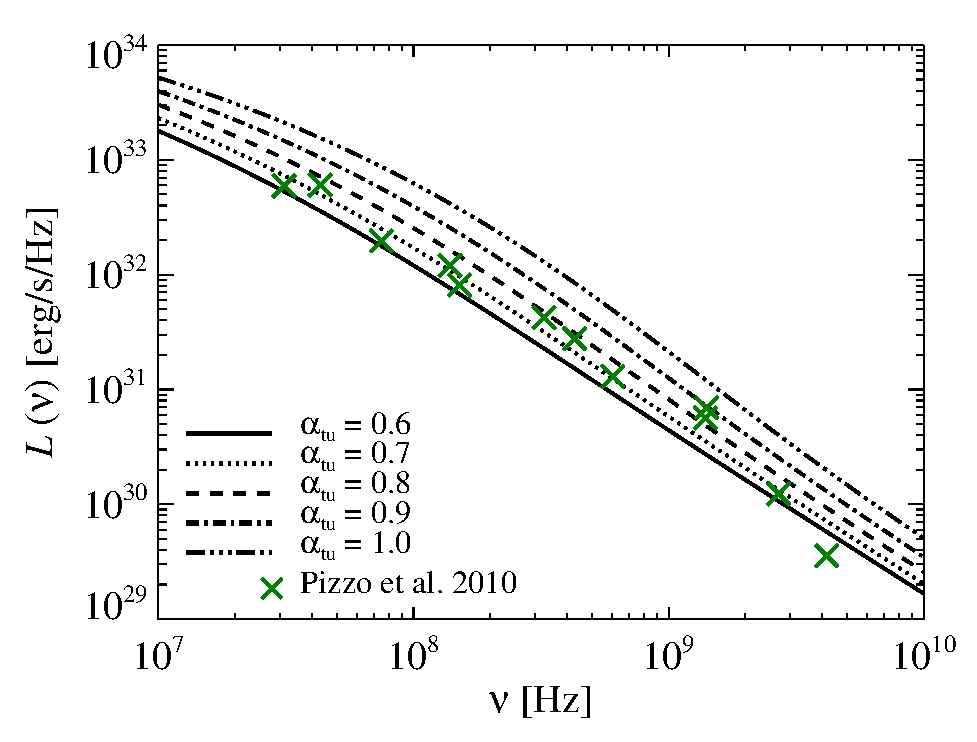
\includegraphics[width=\columnwidth]{spec.comp.KrTTDth.aI0.eps}
   \end{center}
\end{minipage}
\\
\begin{minipage}{1\columnwidth}
  \begin{center}%\Large{\Mflatturb:}\\ 
    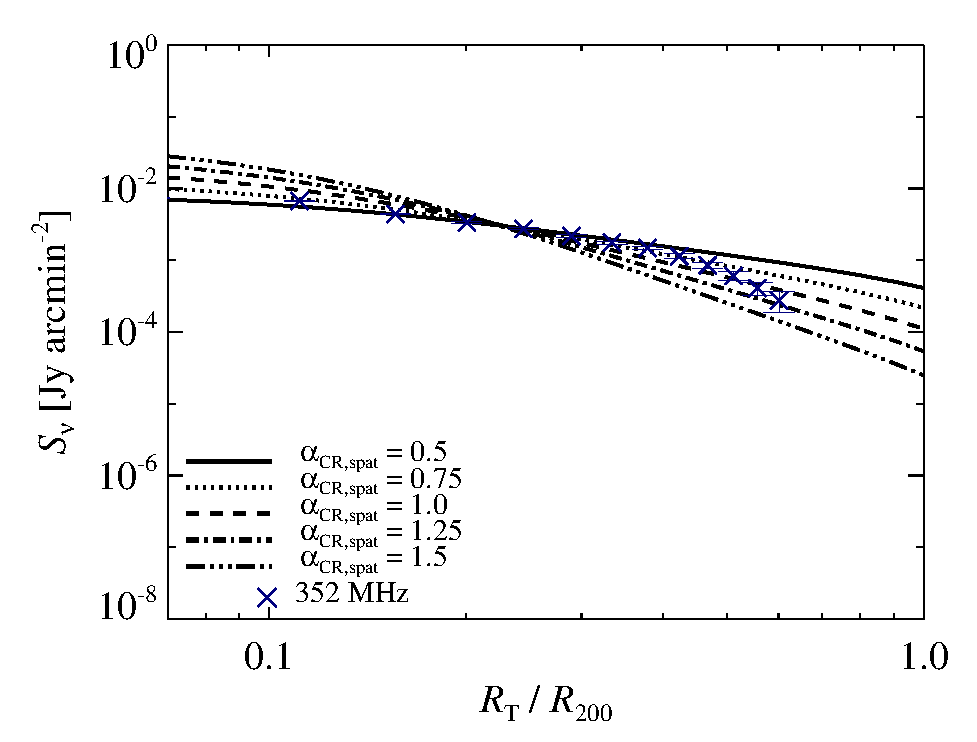
\includegraphics[width=\columnwidth]{prof.comp.KrTTDth.aCR.eps}
  \end{center}
\end{minipage}
\begin{minipage}{1\columnwidth}
   \begin{center}%\Large{\it Brunetti et al. (2012)}:\\
     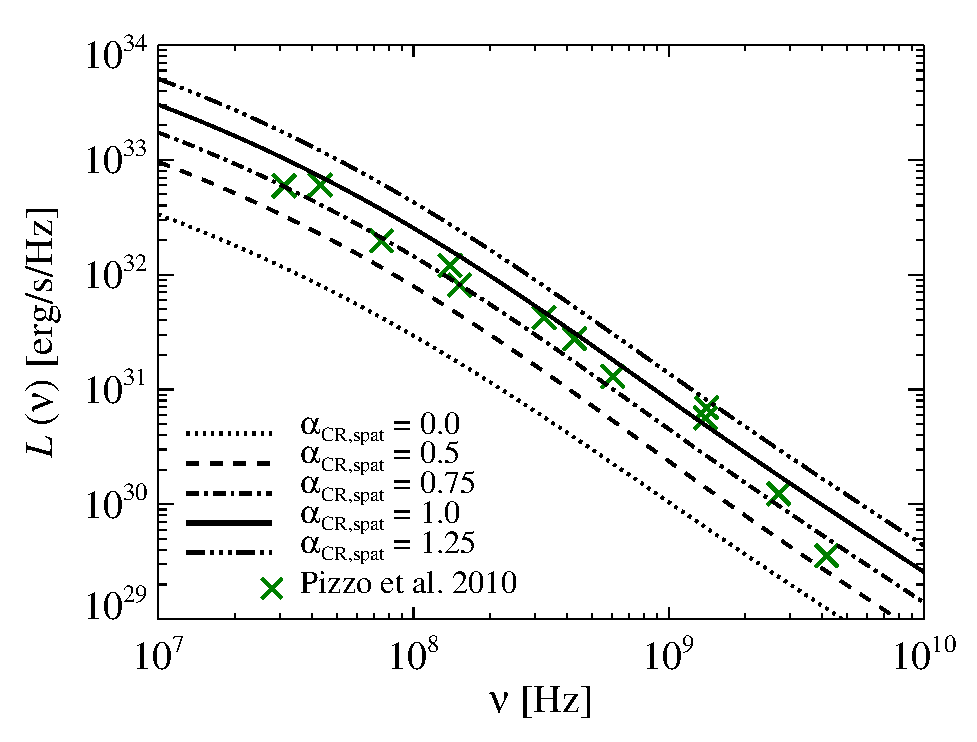
\includegraphics[width=\columnwidth]{spec.comp.KrTTDth.aCR.eps}
   \end{center}
\end{minipage}
\caption{Sensitivity of radio emission in Coma cluster to critical
  parameters. {\it Left panels} show the radio surface brightness
  profiles. We compare profiles at 352~MHz \citep[blue lines and
    crosses,][]{brown11} to predicted emission from Fermi-II
  reaccelerated CR electrons populations (black lines). {\it Right
    panels} show radio synchrotron spectra. The green crosses are
  compiled from observations \citet{2010PhDT.......259P}, while the
  black lines show predicted emission from reaccelerated CR
  electrons. The upper panels show the sensitivity to the level of
  turbulence ($X_\rmn{tu}$), middle panels show the impact of
  different turbulent profiles ($\alpha_\rmn{tu}$), and lower panels
  show the dependence on spatial distributions of initial and injected
  CRs ($\alpha_\rmn{CR,spat}$). We adopt the following fiducial values
  for parameters that are not varied in each panel: $X_\rmn{tu}=0.2$,
  $\alpha_\rmn{tu}=0.8$, and $\alpha_\rmn{CR,spat}=1.0$. Note that the
  radio emission is much more sensitive to assumptions about turbulent
  parameters than CRs.}
  \label{fig:param_comp}
\end{figure*}


% --- section: Simulation Results and discussion --- %
\section{Results of cosmological simulations}
\label{sec:results}

In this section we show that our three models individually reproduce
the observed Coma radio halo without violating gamma-ray bounds. The
level of emission is mainly driven by how efficient the CRs are
reaccelerated and for how long. After turbulent reacceleration, the
volume-weighted, relative CRp energy density and relative CRp number
density inside the RH for \Mflatturb (\Mstream), are found to be 2 (3)
\% and $2\times10^{-8}$ ($5\times10^{-8}$), respectively. As we will
see later, these densities are just of the right order of magnitude to
reproduce radio observations in the Coma cluster. We exploit the large
uncertainty in the turbulent profile and adjust $\alpha_\rmn{tu}$ for
each model so that the CRs have the correct spatial profile to match
the radio emission. The shape of the spectrum for each of model is
more complicated and is determined both from reacceleration and as
well as the gains and losses during the formation of the cluster. It
depends only weakly on the specifics of the CR injection at the shocks
(where the Mach number distribution of the shocks is the most
important quantity). The normalization of the spectrum is mainly
determined from the maximum acceleration efficiency (together with the
uncertain parameters $X_\rmn{tu}$, $\tau_\rmn{cl}$, and $k_0$). Given
the freedom in the turbulens, it might not be surprising that we match
the radio profile in Coma. Although, matching the spectrum without
violating gamma-ray bounds for each of our three models is more
surprising and is not a consequence of parameter fitting. We believe
that it is ultimately a consequence of the adopted physics and hint
that reacceleration is a viable explanation for giant radio
halos. Below we discuss in more detail the different emission
components of Coma.

\subsection{Radio profile}
In Fig.~\ref{fig:sync_profile}, we find that all three scenarios in
which the seeds undergo Fermi-II reacceleration can reproduce the Coma
RH profile at 352~MHz. In the panel {\it Brunetti et al. (2012)} we
show that without CR streaming or a flat turbulent profile, our
simulations of reaccelerated CRs produce radio profiles that are too
steep. Indeed, even using the assumptions of previous work -- where
complete freedom in the seed population was allowed -- it is not
possible to reproduce observations in both frequencies in any
model. Note that decreasing acceleration efficiency with radius does
not change this conclusion much because of the weak radial dependence
of $D_\rmn{pp}(R)\propto
\epsilon_\rmn{th}(R)^{\alpha_\rmn{tu}-1}\sqrt{T(R)}$. This
signals that the problem is generic and requires either additional
modifications to the plasma physics of acceleration or a better
understanding of potential observational systematics. In addition
there are differences in the simulated density and temperature
profiles in comparison to the observed profile in Coma that impact the
CR abundance as well as cooling and reacceleration.

In principle, reacceleration via TTD leads to spectral steepening with
particle energy due to the inefficiency of the acceleration process to
counter the stronger cooling losses with increasing energy. Since
synchrotron emission peaks at frequency $\nu_\rmn{syn}\simeq 1\,
B/\mu\rmn{G} (\gamma/10^4)^2\,\rmn{GHz}$, this translates into a
spectral steepening of the radio spectrum (see
Fig.~\ref{fig:sync_spectrum}). A given radio window samples higher
energy electrons for a decreasing field strength in the cluster
outskirts. Hence, the spectral steepening with energy should translate
into a radial spectral steepening \citep{brunetti12}. However, because
of the weak dependence of the electron Lorentz factor on emission
frequency ($\gamma\propto\sqrt{\nu_\rmn{syn}}$), this effect is only
visible in our simulations for $\nu_\rmn{syn}\gtrsim5$~GHz. Most
importantly, our simulated fluid elements at a given radius sample a
broad distribution of shock history, density and temperature, which
implies very similar synchrotron brightness profiles at
$\nu_\rmn{syn}=352$~MHz and 1.4 GHz. The discrepancy of the observed
and simulated 1.4 GHz profiles could instead be due to systematic flux
calibration error in single dish observations. These could arise, for
instance, due to errors in point source subtraction. Interestingly, we
can match the 1.4 GHz data if we reduce the zero point by adding 10\%
of the central flux to every data point; this flattens the outer
profile\footnote{Lawrence Rudnick, private communication.}.
Alternatively, this may point to weaknesses in the theoretical
modeling of the particle acceleration process and may require a
stronger cutoff in the particle energy spectrum.

\begin{figure*}
\begin{minipage}{1\columnwidth}
   \begin{center}\Large{\Mprimary:}\\
     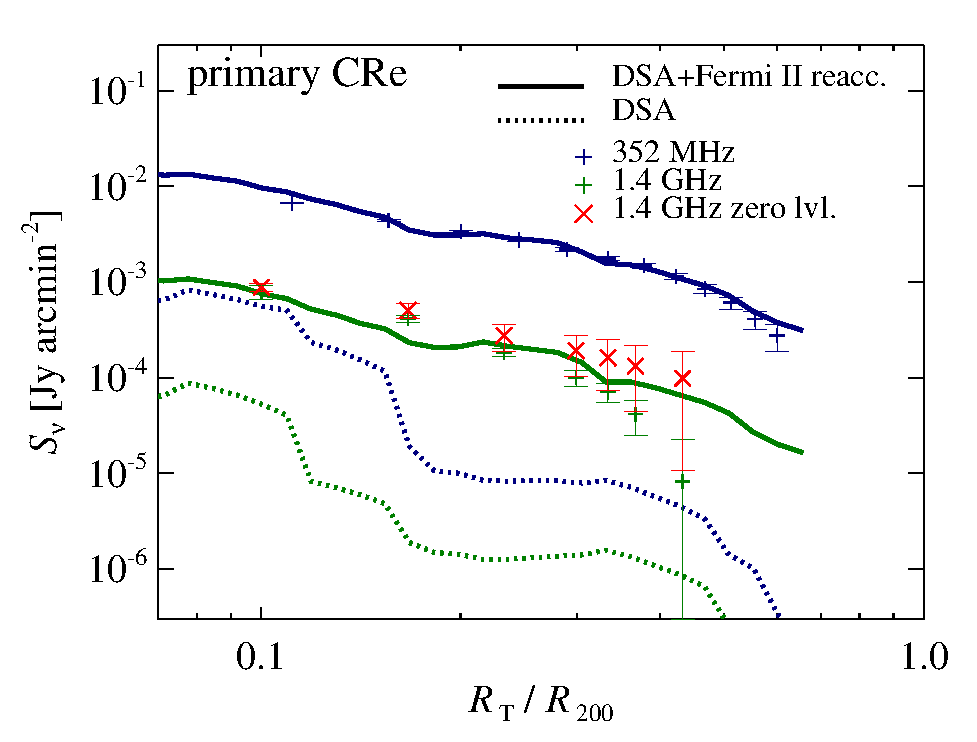
\includegraphics[width=\columnwidth]{sbright.nu.DIIcomp.Pri.g72a.Rad14.2400p.z0.NL.xKR.eb23.eI088.140.v6.eps}
   \end{center}
\end{minipage}
\begin{minipage}{1\columnwidth}
   \begin{center}\Large{\Mstream:}\\
     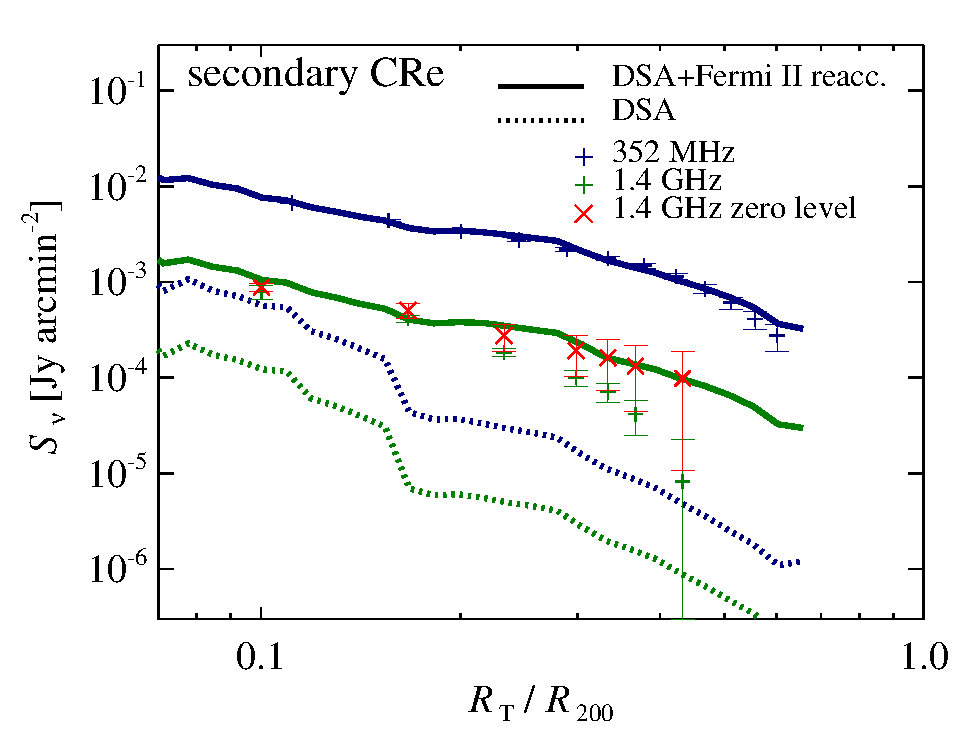
\includegraphics[width=\columnwidth]{sbright.nu.DIIcomp.flatCR.g72a.Rad14.2400p.z0.NL.xKR.eb23.eI082.flatCR.140.v6.eps}
   \end{center}
\end{minipage}
\\
\begin{minipage}{1\columnwidth}
  \begin{center}\Large{\Mflatturb:}\\ 
    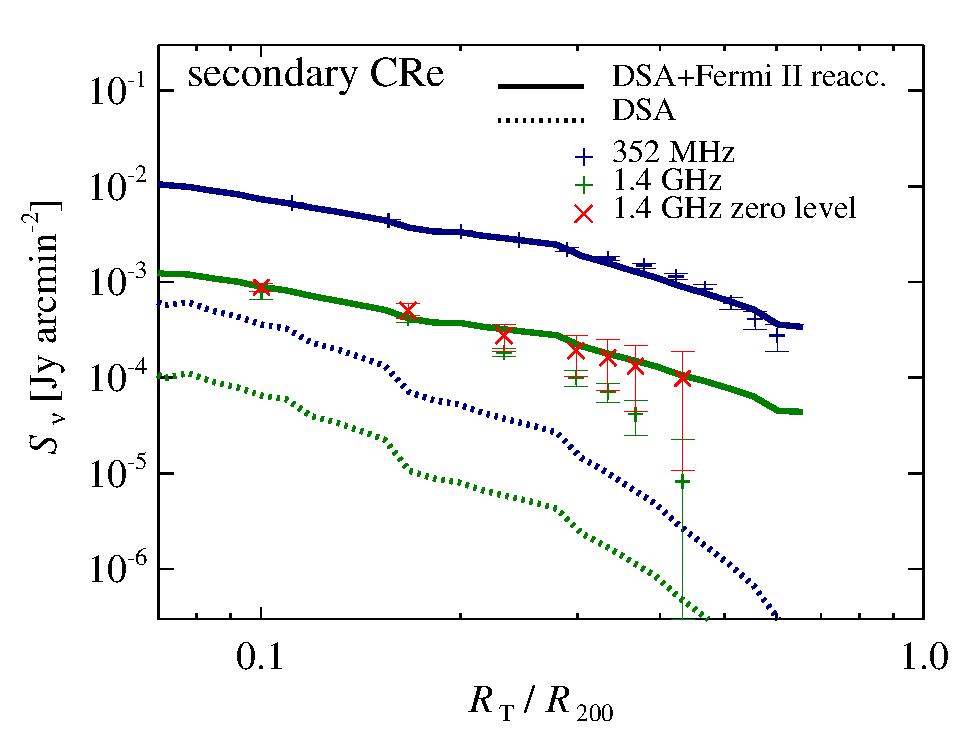
\includegraphics[width=\columnwidth]{sbright.nu.DIIcomp.I0.g72a.Rad14.2400p.z0.NL.xKR.eb23.eI067.140.v6.eps}
  \end{center}
\end{minipage}
\begin{minipage}{1\columnwidth}
   \begin{center}\Large{\it Brunetti et al. (2012)}:\\
     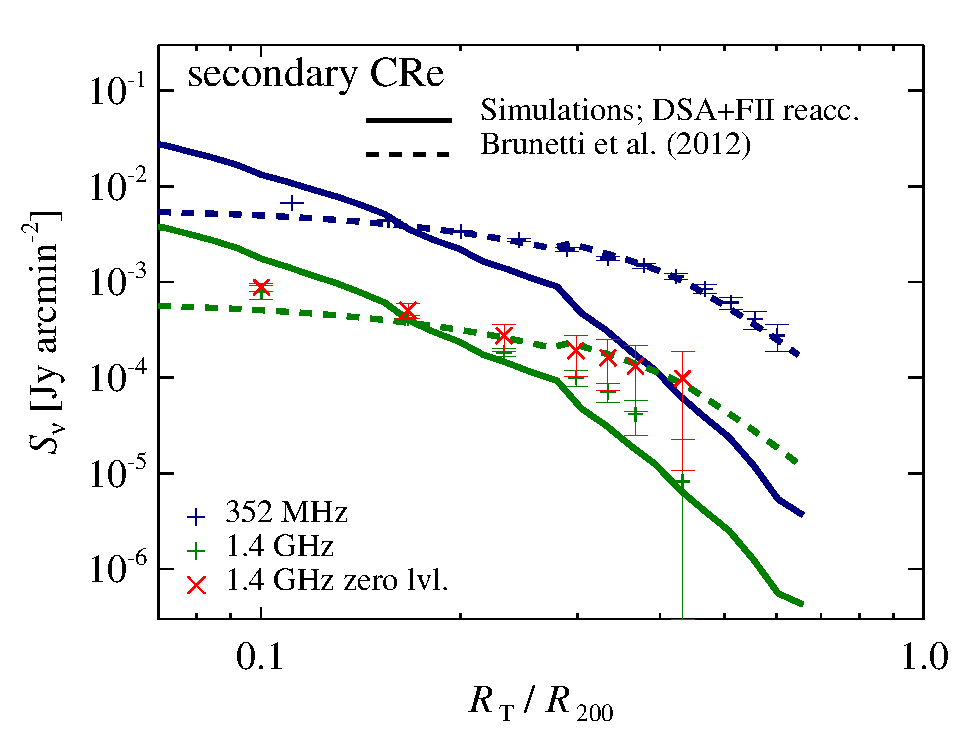
\includegraphics[width=\columnwidth]{sbright.nu.DIIcomp.Brunetti.g72a.Rad14.2400p.z0.NL.xKR.eb23.140.v6.eps}
   \end{center}
\end{minipage}
\caption{Radio surface brightness profiles of Fermi-II reaccelerated
  CR electrons of a simulated post-merging cluster similar to Coma. We
  compare profiles at 352~MHz \citep[blue lines and
    crosses,][]{brown11} to those at 1.4~GHz \citep[green lines and
    crosses,][]{deiss97}. The red crosses show the reprocessed 1.4~GHz
  data, where a zero level of about 10~\% of the central value is
  adopted. The solid lines show predicted emission from a
  reaccelerated fossil population, while dotted lines show emission
  from a fossil population without reacceleration. The panels show the
  emission of our models \Mprimary (upper left panel), \Mstream (upper
  right panel), \Mflatturb (lower left panel), and simulated secondary
  electrons together with previous estimates \citep{brunetti12} for
  the Coma cluster (lower right panel).}
  \label{fig:sync_profile}
\end{figure*}

\subsection{Radio spectrum}
\label{sect:radio_spec}
In Fig.~\ref{fig:sync_spectrum} we show that our three models that
include Fermi-II reacceleration can individually reproduce the
convexly curved total radio spectrum found in the Coma cluster. Seed
CRs in \Mstream and \Mflatturb that do not experience turbulent
reacceleration have a power-law spectrum in disagreement with
observations. In order to match both the spatial and spectral profiles
in Coma, we adopt an acceleration efficiency for the strongest shocks
in our three models \Mprimary, \Mstream, and \Mflatturb to
$\zeta_{\rmn{e}} <0.003$, $\zeta_{\rmn{p}} < 0.1$, and
$\zeta_{\rmn{p}}<0.03$, respectively. Following the Mach number
($\mathcal{M}$)-dependence of the acceleration efficiency suggested in
\cite{pinzke13}, the efficiency in weak shocks ($\mathcal{M}\sim
2.5-3.5$) that dominates the CR distribution function, has an
acceleration efficiency for protons $\zeta_{\rmn{p}}\sim0.0001-0.01$,
and for electrons $\zeta_{\rmn{e}}\sim 0.001$. Interestingly, we find
that the radio luminosity from clusters in the OFF-state (DSA only)
and ON-state (DSA and reacceleration) differ by about a factor 10 in
all our three models. However, note that for \Mprimary, the primary
CRes that generate most of the radio emission from the cluster in the
OFF-state are dominated by only a small fraction of the CRes. These
electrons are injected very recently and have not had time to cool
yet. Hence we expect there to be a large variance in the OFF-state of
different simulated clusters. As mentioned in
section~\ref{sect:param_comp}, combining radio observations with
gamma-ray limits allows us to put a lower limit to $X_\rmn{tu}$.  If
$X_\rmn{tu}$ is smaller than in our adopted models (where we assume
$X_\rmn{tu}=0.2$), then the efficiency of DSA has to be larger than
$\zeta_\rmn{p}\sim 0.1$ for the secondary CRes to reproduce the radio
observations. However, since the turbulent reacceleration acts on both
the secondary CRes and the CRps, while $\zeta_\rmn{p}$ only affects
the CRps, \Mstream and \Mflatturb would produce too much
gamma-rays. Hence we conclude that $X_\rmn{tu}\gtrsim0.2$ if all other
parameters are kept fixed. Although, we caution the reader to take
this limit too stringent because of the uncertainty in $k_0$ and
$\tau_\rmn{cl}$ that impact $X_\rmn{tu}$ for a fixed
$\tau_\rmn{D}$. This parameter space needs to be explored further in
future work in order to put more stringent limits on the level of
turbulence in clusters using radio and gamma-ray observations in
combination with turbulent reaccelerated CRs.

\begin{figure*}
  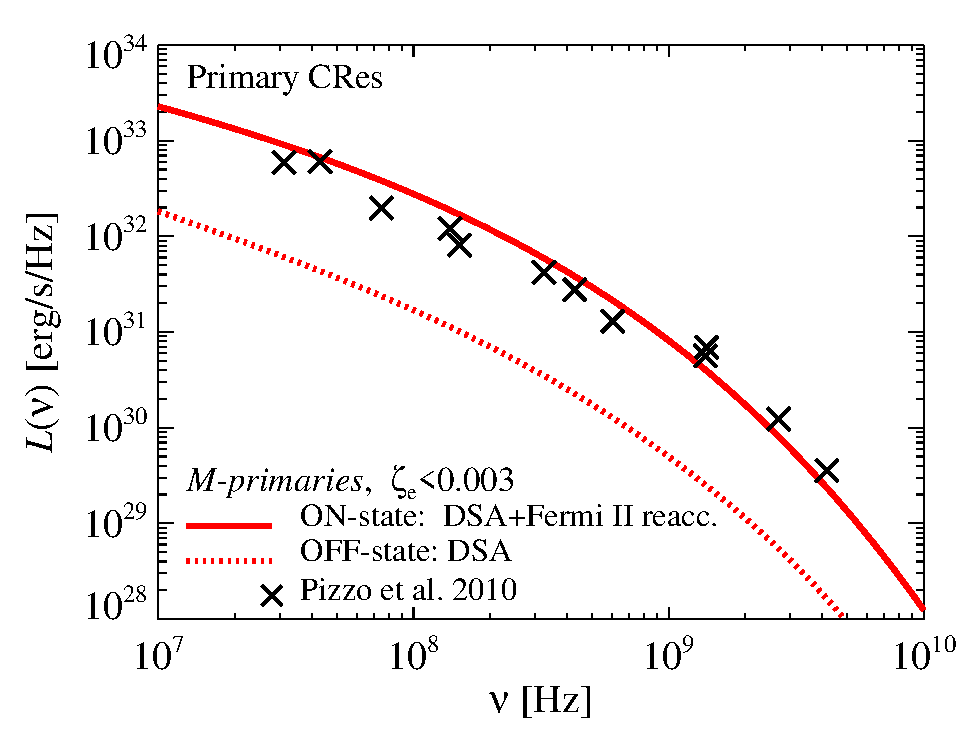
\includegraphics[width=1.0\columnwidth]{sync.spec.pri.g72a.140.v6.eps}
  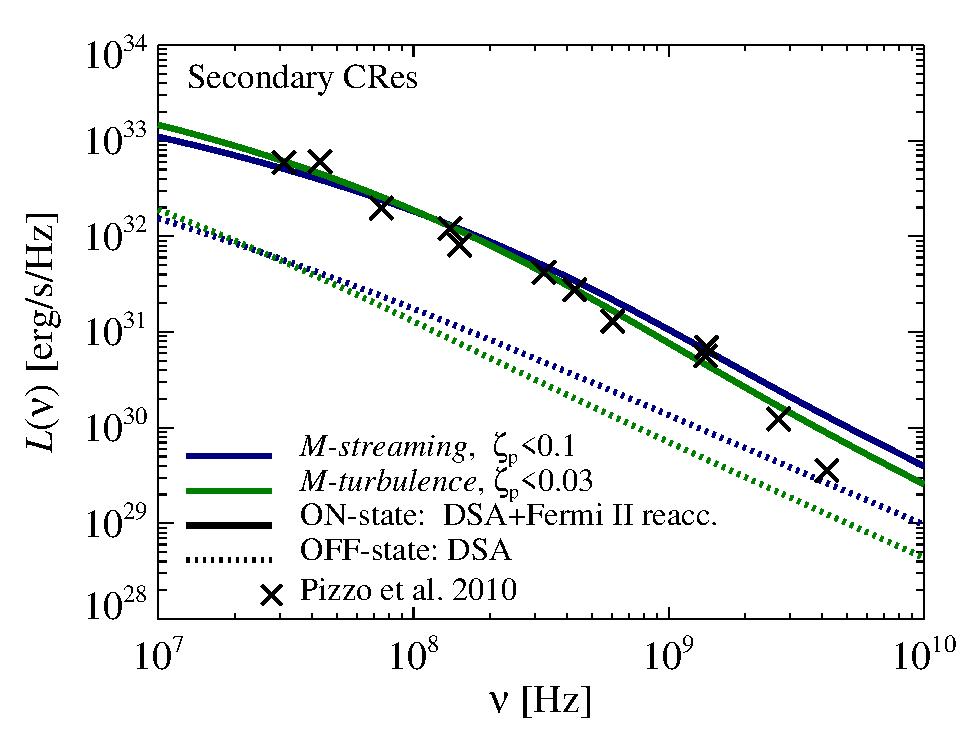
\includegraphics[width=1.0\columnwidth]{sync.spec.sec.g72a.140.v6.eps}
  \caption{Radio synchrotron spectra. Lines are derived from
    simulations, while the black crosses are compiled from
    observations \citet{2010PhDT.......259P}. The solid lines show the
    DSA and reaccelerated CRs (On-state of the radio halo), while the
    dotted lines show CRs accelerated only by DSA (Off-state of the
    radio halo). The left figure shows the radio emission induced by
    primary CRes and the right figure shows the emission from
    secondary CRes. The different line colors represent our different
    models, \Mprimary (red line), \Mstream (blue line), and \Mflatturb
    (green line).}
  \label{fig:sync_spectrum}
\end{figure*}

\subsection{Gamma-rays}
The gamma-ray emission from CRps that produce decaying neutral pions
could be substantial if the CRps are reaccelerated efficiently enough,
hence it is interesting to estimate this emission for our models and
compare to upper limits. We predict the gamma-ray emission from
\Mflatturb (\Mstream) with $F_\gamma(>500\,\rmn{MeV})=4\times10^{-10}
(5\times10^{-10}) \mathrm{ \,ph\, s}^{-1}\mathrm{cm}^{-2}$. The fluxes
from these models are slightly larger than in \cite{brunetti12}, where
the differences comes from our steeper CRp profiles in addition to
simulation based formalism we rely on that accounts for both Coulomb
and hadronic losses during the build up of the CR distribution in
contrast to the scaling relations adopted in their
paper. Interestingly the gamma-ray flux from both our scenarios are
just below recent Fermi-LAT limits derived from a gamma-ray profile
similar to \Mflatturb where
$F_\gamma(>500\,\rmn{MeV})<5.3\times10^{-10} \mathrm{ \,ph\,
  s}^{-1}\mathrm{cm}^{-2}$ \footnote{Fabio Zandanel, private
  communication. See also
  \citet{2014MNRAS.440..663Z,2014ApJ...787...18A}. and will be probed
  in the next few years by Fermi-LAT. } The spectral index of the CRp
distribution is relatively steep ($\alpha_{\rmn{p}}\sim2.6$) for the
CRp energies $E \gtrsim 10$~GeV that are relevant for the injection of
radio-emitting secondary CRes. The steep spectrum is ultimately a
consequence of the shock history of the simulated cluster, with a weak
dependence on our test particle model for Fermi-I acceleration
\citep{pinzke13}, where we steepen the spectral index to avoid
acceleration efficiencies above $\zeta_{\rmn{p}} \sim 10\%$.


% --- section: Conclusions --- %
\section{Conclusions}
\label{sec:conclusions}

The standard reacceleration model for radio halos (RHs) requires a
population of seed electrons to undergo turbulent
reacceleration. These seeds are generally thought to be secondary
electrons from hadronic cosmic ray proton (CRp) interactions. In this
work we use cosmological simulations to derive a population of seed CR
protons originating from structure formation shocks and merger shocks
during the cluster build up. The resulting secondary population is
inconsistent with RH observations. We propose three possible solutions
where all reaccelerated CRs produce gamma-ray emission below current
upper limits. Additionally, they reproduce both the spectrum and the
surface brightness profiles of the Coma radio halo:

\begin{enumerate}
\item {\bf Model {\em M-primaries}.} If indeed the acceleration
  efficiency of CRps is below about $0.1$ {\%} in weak shocks and the
  ratio of injected electrons and protons is $K_{\rmn{ep}} \sim
  10^{-1}$, CR electrons accelerated directly in shocks dominate over
  secondaries.
\item {\bf Model {\em M-streaming}.} Alternatively, CRps could stream
  out of the central core and produce flat CR profiles. This seed
  population of secondary CRes also has the correct spatial and
  spectral features alone, or potentially complements primaries to
  explain radio observations.
\item {\bf Model {\em M-turbulence}.}  Finally, injected turbulence
  that is flatter than in previously adopted models, which allows seed
  CRps to follow the steep radial profile that is suggested by
  structure formation simulations.
\end{enumerate}

Combining radio observations with gamma-ray constraints can be very
useful to learn about the plasma of the intracluster medium. Our
models (ii) and (iii) relies on CRps to induce secondary CRes that
produce the observed radio emission. In addition proton-proton
collisions produce neutral pions that decay into gamma rays. Since
turbulent reacceleration acts on both CRes and CRps, while the DSA
acceleration efficiency ($\zeta_p$) only acts on the CRps, radio
observations fix the relation between $X_\rmn{tu}$ (the ratio of the
total turbulent energy in compressional modes to the total thermal
energy) and the acceleration efficiency. With the addition of
gamma-ray constraints from Fermi-LAT, we can derive a lower limit to
$X_\rmn{tu}\gtrsim0.2$ and a upper limit to the acceleration
efficiencies of $\zeta_p\lesssim 10\%$ ($\zeta_p\lesssim 3\%$) for
the two models, respectively, for our current choices of other
parameters.

How could we distinguish the different possibilities of a dominating
primary or secondary seed population of electrons observationally?
One possibility that is relative insensitive to adopted parameters in
our models is to use high-frequency radio observations (with e.g., the
Jansky Very Large Array) where turbulent reacceleration (which has a
high energy cutoff) is no longer efficient (see
Fig.~\ref{fig:sync_spectrum}). The negative flux bowl of the
Sunyaev-Zel'dovich effect introduces a cutoff of the RH spectrum at
frequencies above $\gtrsim 10$~GHz \citep[][ depending on cluster mass
  and redshift]{2002A&A...396L..17E,Pfrommer:2003mk}. Hence the
subdominant hadronic radio emission may only be detectable in steep
spectrum radio sources \citep{2008Natur.455..944B}, which exhibit a
cutoff at lower radio frequencies and are thought to represent dying
RHs as a result of the decaying turbulence after a
merger. Alternatively, one could attempt to reconstruct the intrinsic
high-frequency RH spectrum by filling in the missing flux due to the
Sunyaev-Zel'dovich effect by precise measurements of the Compton-$y$
parameter at microwave frequencies. Another possibility would consist
in stacking the radio data of radio-quiet clusters that due not
exhibit RH emission \citep{2011ApJ...740L..28B}. This may reveal the
glow of radio emission due to steady state secondary
population. Emission from faint secondary electrons should still be
visible, whereas due to the much more intermittent nature of DSA
injection, primary CRe will instead show a sharp cutoff due to
cooling, and will not be visible at high energies (see
Fig.~\ref{fig:sync_spectrum}). We will pursue further implications and
distinguishing characteristics of these competing models in future
work.

{\bf Acknowledgments.} We thank Josh Wiener for discussions on CR
streaming. We are also grateful to Lawrence Rudnick for discussion on
uncertainties in the 1.4 GHz radio data. Finally, we thank Fabio
Zandanel for recalculating gamma-ray limits and Gianfranco Brunetti
for useful discussions. A.P. is grateful to the Swedish research
council for financial support. S.P.O. thanks NASA grant NNX12AG73G for
support. C.P.~gratefully acknowledges financial support of the Klaus
Tschira Foundation.
%%%%%%%%%%%%%%%%%%%%%%%%%%%%%%%%%%%%%%%%%%%%%%%%%%%%%%%%%%%%%%%
\vspace{-0.7cm}

\bibliography{paper}
\bibliographystyle{mnras}

\end{document}
